%http://texblog.org/2011/09/09/10-ways-to-customize-tocloflot/

%Автоматически вписывать картинки в ширину страницы:
%\includegraphics[maxwidth=\linewidth]{foobar}

\if 0
Так можно сделать многострочный комментарий.
Это маленький хак. Его надо использовать.
\fi

\documentclass[twoside,11pt,a4paper,notitlepage]{report}

\makeatletter
\newcommand*{\toccontents}{\@starttoc{toc}}
\usepackage{pscyr}
\usepackage[T2A]{fontenc}
\usepackage[utf8]{inputenc}
\renewcommand{\rmdefault}{CMR}
\usepackage[russian]{babel}
\usepackage[dvipsnames]{xcolor}

%\usepackage{classicthesis}
%\usepackage[toctitles]{titlesec}
\usepackage{listings}

\usepackage{titlesec}



% Создание индекса
%\usepackage{makeidx}
%\makeindex

%История изменений
%\usepackage{vhistory}
\usepackage[owncaptions]{vhistory}%[tocentry] включить в оглавление


\usepackage[most]{tcolorbox} % для управления цветом
\definecolor{block-gray}{gray}{0.90} % уровень прозрачности (1 - максимум)
\newtcolorbox{myquote}{colback=block-gray,grow to right by=-10mm,grow to left by=-10mm,
	boxrule=0pt,boxsep=0pt,breakable} % настройки области с изменённым фоном

%*************************
\usepackage{shorttoc}% Краткое оглавление
%*************************

%*************************
\usepackage{tocloft}% Управление оглавлением
%*************************



%Fncychar позволит выбрать несколько различных стилей, красиво оформляющих наименование глав.
%\usepackage[Glenn]{fncychap} % выбираем стиль Glenn

%Пакет titlesec позволяет вносить изменения в стандартный стиль главы, то есть переопределять его.
%\usepackage{titlesec, blindtext, color} % подключаем нужные пакеты
%\definecolor{gray75}{gray}{0.75} % определяем цвет
%\newcommand{\hsp}{\hspace{20pt}} % длина линии в 20pt
%% titleformat определяет стиль
%\titleformat{\chapter}[hang]{\Huge\bfseries}{\thechapter\hsp\textcolor{gray75}{|}\hsp}{0pt}{\Huge\bfseries}

\usepackage{listings}      % для кусков программ 
% (понимает синтаксис некоторых языков, чума просто)
\usepackage{alltt}         % для того же
\usepackage{amssymb}       % прикольно для формул

\pagestyle{plain} % нумерация страниц вкл.

%http://tex.stackexchange.com/questions/181183/combine-usepackagetimes-and-fontspec-setmainfont
%http://andreyolegovich.ru/PC/LaTeX.php#base

%********************
% Набор предоставляет дополнительные математические символы, множество удобных возможностей для оформления математических формул (например, упрощённую работу с многострочными формулами) и используется почти во всех LaTeX-документах, в которых есть сколько-нибудь сложные формулы.
%******************** 
\usepackage{amsmath}



\usepackage{titlesec}
\usepackage{csquotes} % ещё одна штука для цитат

\usepackage{sectsty}
%\subsectionfont{\Large\underline}
\subsectionfont{\Large}

\usepackage{graphicx}
\usepackage{sidecap}
\usepackage{xcolor}
\usepackage{pdfpages}
\usepackage{comment}
\usepackage{textcomp}
\usepackage{wrapfig}
\usepackage{sectsty}
\usepackage{lipsum}
\usepackage{fancyhdr}
\usepackage{datetime}
\chapterfont{\centering}

\usepackage{caption}
\usepackage{subcaption}

\usepackage[T2A]{fontenc}
\usepackage{lscape}
\usepackage{makecell}
\usepackage{multicol}
\usepackage{floatrow}
\usepackage{float}
\usepackage{caption}
\usepackage{lastpage} % Allows referencing of the last page to allow footer to read: "Page [Current page] of [Total number of pages]."

\renewcommand{\familydefault}{\sfdefault} %Изменит стандартный шрифт документа на сансерифный.

\definecolor{MSBlue}{rgb}{.204,.353,.541}
\definecolor{MSLightBlue}{rgb}{.31,.506,.741}
%\titleformat*{\section}{\Large\bfseries\sffamily\color{MSBlue}}
%\titleformat*{\subsection}{\large\bfseries\sffamily\color{MSLightBlue}}
%\titleformat*{\subsubsection}{\itshape\subsubsectionfont}

\titleformat
{\chapter} % command
[display] % shape
{\bfseries\Large\itshape} % format
{Story No. \ \thechapter} % label
{0.5ex} % sep
{
	\rule{\textwidth}{1pt}
	\vspace{1ex}
	\centering
} % before-code
[
\vspace{-0.5ex}%
\rule{\textwidth}{0.3pt}
] % after-code


\titleformat{\section}[wrap]
{\normalfont\bfseries}
{\thesection.}{0.5em}{}

\titlespacing{\section}{12pc}{1.5ex plus .1ex minus .2ex}{1pc}





%*****************************************************
% Часто требуется, чтобы номер рисунка содержал в себе номер главы (вроде Рис. 1.1). Чтобы была сделана нумерация по главам, достаточно изменить счётчик рисунков в преамбуле документа вот так:
\renewcommand{\thefigure}{\thesection.\arabic{figure}}
%*****************************************************

%*****************************************************
%Если вас не устраивает вид подрисуночной подписи (например, вместо "Рис. 1:" необходимо "Рис. 1 --- "), используйте пакет caption. В частности, для установки тире в качестве разделителя, вставьте в преамбулу документа следующий код: 
\RequirePackage{caption}
\DeclareCaptionLabelSeparator{defffis}{ --- }
\captionsetup{justification=centering,labelsep=defffis}
%*****************************************************

%\usepackage[colorlinks=true,linkcolor=blue]{hyperref}

%*****************************************************
%Как сделать, чтобы уравнения нумеровались независимо по главам в LaTeX?
%В преамбуле
\makeatletter \@addtoreset{equation}{section} \makeatother 
\makeatletter \@addtoreset{figure}{section} \makeatother 
%*****************************************************

\addto\captionsrussian{
	\def\figurename{Рисунок}
}


\usepackage[hypcap]{caption}

%*****************************************************
% Начинать секции с новой страницы
\usepackage{titlesec}
\newcommand{\sectionbreak}{\clearpage}
%*****************************************************


%*****************************************************
%Чтобы в генерированном PDF работали гиперссылки, то надо подключить модуль hyperref (и если хотите их разрисовать, то модуль по работе с цветами xcolor):
\usepackage{hyperref}
% Цвета для гиперссылок
\definecolor{linkcolor}{HTML}{012b37} % цвет ссылок
\definecolor{urlcolor}{HTML}{012b37} % цвет гиперссылок
\hypersetup{pdfstartview=FitH,  linkcolor=linkcolor,urlcolor=urlcolor, colorlinks=true}
%*****************************************************

%***************************************************** 
%Для удаления номеров страниц из \listoffigures
\makeatletter
\newcommand{\emptypage}[1]{%
	\cleardoublepage
	\begingroup
	\let\ps@plain\ps@empty
	\pagestyle{empty}
	#1
	\cleardoublepage}
\makeatletter
%*****************************************************


\setcounter{secnumdepth}{3}
%\usepackage{enumitem}
\usepackage[shortlabels]{enumitem}
\setlist[enumerate]{leftmargin=*,align=left,label=\thesubsection.\arabic*.}
%\usepackage{enumerate}
\usepackage{longtable}

%\renewcommand{\rmdefault}{ftm}
\renewcommand{\rmdefault}{cmr}
\renewcommand{\thesection}{\arabic{section}}
%\usepackage{enumitem}
%%% Страница
%\usepackage{extsizes} % Возможность сделать 14-й шрифт
\usepackage{geometry} % Простой способ задавать поля
\geometry{top=15mm}
\geometry{bottom=10mm}
\geometry{left=10mm}
\geometry{right=10mm}

%*****************************************************
%Here is how you can increase the space between the number and the caption in your \listoffigures. Add the following two lines before your \begin{document}:
\usepackage{tocloft}
\setlength{\cftfignumwidth}{3em}
%With the tocloft-package you can control the design of table of contents, figures and tables.
%*****************************************************

% раскомментировать, чтобы увидеть забавную картинку размещения текста
%\usepackage{layout}
% увидеть, что не сработало и раскомментировать \layout внизу
%%%%%%%%%%%%%%%%%%%%%%%%%%%%%%%%%%%%%%%%%%%%%%%%%%%%%%%%%%%%%%%%%%%%%%%%%%%%%%%%


%%%%%%%%%%%%%%%%%%%%%%%%%%%%%%%%%%%%%%%%%%%%%%%%%%%%%%%%%%%%%%%%%%%%%%%%%%%%%%%%
%%%
%%% мелочи жизни (переопределение буллетов для списков)
%%%
\renewcommand{\labelitemii}{{$\mathbf{+}$}}
\renewcommand{\labelitemiii}{{$\mathbf{++}$}}

%%%%%%%%%%%%%%%%%%%%%%%%%%%%%%%%%%%%%%%%%%%%%%%%%%%%%%%%%%%%%%%%%%%%%%%%%%%%%%%%
%%%
%%% Моя любимая настройка параметров страницы. По умолчанию колонка узковатая
%%%
\voffset=-10mm
\topmargin=0mm
\headheight=5mm
\headsep=10mm

\textheight=237mm
\footskip=10mm

\oddsidemargin=-2mm
\evensidemargin=-15mm
% регулирует расстояние sidenotes от края страницы
\hoffset=5mm
\textwidth=175mm
\marginparsep=10mm
%%%%%%%%%%%%%%%%%%%%%%%%%%%%%%%%%%%%%%%%%%%%%%%%%%%%%%%%%%%%%%%%%%%%%%%%%%%%%%%%

\usepackage{caption}

\usepackage{svn}


\pagestyle{fancy}
%\fancyfoot[]{вер. 1.05}

%\fancyhead[C]{Страница \thepage \; из \pageref{LastPage}}
%\fancyhead[RE]{\slshape\nouppercase{\rightmark}}
%\fancyhead[LO]{\slshape\nouppercase{\leftmark}}
%\fancyfoot[C]{Страница \thepage \; из \pageref{LastPage}}
%\renewcommand{\headrulewidth}{0pt}
%\renewcommand{\footrulewidth}{0pt}
%\lhead{\footnotesize \parbox{11cm}{Draft 1} }

% Allows calling chapter and section names in headers and footers.
%\renewcommand{\chaptermark}[1]{%
%	\markboth{\chaptername\ \thechapter}
%	{\noexpand\firstsubsectiontitle}}
%\renewcommand{\sectionmark}[1]{}
%\renewcommand{\subsectionmark}[1]{%
%	\markright{#1}\gdef\firstsubsectiontitle{#1}}
%\newcommand\firstsubsectiontitle{}



\lhead{\footnotesize \parbox{11cm}}
%\lfoot{\footnotesize \parbox{11cm}{\textit{2}}}
%\cfoot{}
\rhead{\footnotesize  \chaptername \ - \rightmark}
%\rfoot{\footnotesize Page \thepage\ of \pageref{LastPage}}
%\fancyfoot[C]{Страница \thepage \; из \pageref{LastPage}}
\fancyfoot{} % Clear all footer fields
\fancyfoot[RO,L] {v.\vhCurrentVersion \ \vhCurrentDate}  % Версия и дата
\fancyfoot[RO,R]{Страница \thepage \; из \pageref{LastPage}} % Page number on right in footer

%\renewcommand{\headheight}{24pt}
\setlength{\headheight}{4pt}
\renewcommand{\footrulewidth}{0pt}
%\setlength\headheight{80.0pt}
%\addtolength{\textheight}{-80.0pt}
%\chead{\includegraphics[width=\textwidth]{img/log1o.png}}
%\cfoot{\includegraphics[width=\textwidth]{img/foot.png}}

\graphicspath{{images/}}



%*****************************************************
%Номера страниц, включающие номер главы
\usepackage[auto]{chappg} %%% this is to set the page numbers as Chapter-Page.
%*****************************************************



\newdate{date}{28}{01}{2016}
\date{\displaydate{date}}
%Increase the value of tocdepth and secnumdepth. The tocdepth value determines to which level the sectioning commands are printed in the ToC (they are always included in the .toc file but ignored otherwise). The secnumdepth value determines up to what level the sectioning titles are numbered. They are LaTeX counters and you can set them using 
\setcounter{tocdepth}{1}
\setcounter{secnumdepth}{4}

\renewcommand{\theenumi}{\arabic{enumi}}
\renewcommand{\labelenumi}{\arabic{enumi}}
\renewcommand{\theenumii}{.\arabic{enumii}}
\renewcommand{\labelenumii}{\arabic{enumi}.\arabic{enumii}.}
\renewcommand{\theenumiii}{.\arabic{enumiii}}
\renewcommand{\labelenumiii}{\arabic{enumi}.\arabic{enumii}.\arabic{enumiii}.}


\usepackage{titlepic}



%\titlespacing\section{0pt}{12pt plus 4pt minus 2pt}{0pt plus 2pt minus 2pt}
%\titlespacing{\subsection}{0pt}{\parskip}{-\parskip}

\def\capfigure{figure}

\def\captable{table}

\long\def\@makecaption#1#2{%
	
	\vskip\abovecaptionskip
	
	\ifx\@captype\capfigure
	
	\centering #1~--~#2 \par
	
	\else
	
	#1~--~#2 \par
	
	\fi
	
	\vskip\belowcaptionskip}

\setlength\abovecaptionskip{2\p@}

\setlength\belowcaptionskip{1\p@}



%%%%%%%%%%%%%%%%%%%%%%%%%%%%%%%%%%%%%%%%%%%%%%%%%%%%%%%%%%%%%%%%%%%%%%%%%%%%%%%%
%%%
%%% маленький хак, новое окружение 'algorithm' (см. использование ниже)
%%%
\newlength{\algboxsp}
\setlength{\algboxsp}{2mm}
\newsavebox{\algbox}
\newenvironment{basealgorithm}
{\begin{lrbox}{\algbox}\begin{minipage}{\textwidth}\begin{alltt}}
			{\end{alltt}\end{minipage}\end{lrbox}
	\fbox{
		\parbox{0.95\textwidth}{
			\makebox[0mm]{}
			\\[\algboxsp]
			\mbox{\hspace{\algboxsp}}
			\usebox{\algbox}
			\\[\algboxsp] } }}

\newenvironment{algorithm}[1]
{\begin{figure}[btp]\def\algcptn{\caption{#1}}\begin{basealgorithm}}
		{\end{basealgorithm}\algcptn\end{figure}}
	
	
	
%**********************************
% Todo notes - example from http://www.texample.net/tikz/examples/todo-notes/
\usepackage{verbatim}
\usepackage[colorinlistoftodos]{todonotes}
%**********************************

%\usepackage{sidenotes}


\usepackage{geometry}

\usepackage{snotez}



%**********************************************************

% Vertically aligning a marginnote and a section title
%**********************************************************
\usepackage{lipsum}

\usepackage{marginnote}
\reversemarginpar % To put the margin pars on the left
\renewcommand*{\marginfont}{\normalfont\normalsize}

\usepackage{tikz}
\usetikzlibrary{calc}
\usetikzlibrary{backgrounds}

\newcommand*{\Date}[4]{%
	\begin{tikzpicture}[show background rectangle,inner frame sep=0pt,text width=1cm,align=center]
	\node [fill=orange] at (0,0)                                (dayofweek)  {#1};
	\node [fill=white ] at ($(dayofweek)  +(0,-\baselineskip)$) (dayofmonth) {#2};
	\node [fill=white ] at ($(dayofmonth) +(0,-\baselineskip)$) (month)      {#3};
	\node [fill=orange] at ($(month)      +(0,-\baselineskip)$) (dayofmonth) {#4};
	\end{tikzpicture}
}

%**********************************************************
\usepackage{geometry}
\usepackage{marginnote}





	
\renewcommand{\cftchapfont}{\scshape}
\renewcommand{\cftsecfont}{\bfseries}
%\renewcommand{\cftfigfont}{Figure }
%\renewcommand{\cfttabfont}{Table }
	
\usepackage{eso-pic}	


\AddToShipoutPicture{%

	\AtPageLowerLeft{%
		\hspace*{.02\textwidth}%
		\rotatebox{90}{%
			\begin{minipage}{\paperheight}
				\fontsize{6}{6}\selectfont
				%				\centering\textcopyright~\today{} ТД Крюгер
					\textcopyright~ ТД Крюгер
	%				\textcopyright~ ТД Крюгер тел.техподдержки 8-913 016 0854
			\end{minipage} %
		}
	} %
}%

%How can I put real notes in the margin?
%**********************************************************	
\usepackage{xparse}
\usepackage{tikz}
\usetikzlibrary{calc,fit, decorations.pathmorphing}

\makeatletter
% http://tex.stackexchange.com/questions/39296/simulating-hand-drawn-lines
\pgfdeclaredecoration{penciline}{initial}{
	\state{initial}[width=+\pgfdecoratedinputsegmentremainingdistance,auto corner on length=1mm,]{
		\pgfpathcurveto%
		{% From
			\pgfqpoint{\pgfdecoratedinputsegmentremainingdistance}
			{\pgfdecorationsegmentamplitude}
		}
		{%  Control 1
			\pgfmathrand
			\pgfpointadd{\pgfqpoint{\pgfdecoratedinputsegmentremainingdistance}{0pt}}
			{\pgfqpoint{-\pgfdecorationsegmentaspect\pgfdecoratedinputsegmentremainingdistance}%
				{\pgfmathresult\pgfdecorationsegmentamplitude}
			}
		}
		{%TO 
			\pgfpointadd{\pgfpointdecoratedinputsegmentlast}{\pgfpoint{1pt}{1pt}}
		}
	}
	\state{final}{}
}
\makeatother
\newcommand{\tikzmark}[1]{\tikz[overlay,remember picture] \node (#1) {};}
\newcommand{\CommentText}[3]{\tikzmark{#1}#3\tikzmark{#2}}
\NewDocumentCommand{\CommentPar}{%
	O{}% #1 = draw options for the referenced word
	O{}% #2 = draw options for the comment
	O{}% #3 = draw options for the connecting line
	m  % #4 = left \tikzmark name
	m  % #5 = left \tikzmark name
	m  % #6 = comment
}{%
	\begin{tikzpicture}[overlay,remember picture,decoration=penciline, thick]
	\node [shape=rectangle,inner sep=0, draw=blue, ,rounded corners=2pt, fit={(#4.south) ($(#5.north)+(0,0.75ex)$)}, decorate, #1] (Source) {};
	\node at ($(#4)!0.5!(#5)$) [blue, font=\itshape, rounded corners=5pt, decorate, #2] (Label) {#6};
	\draw [draw=red, decorate, #3] (Label) to (Source);
	\end{tikzpicture}
}

%**********************************************************
\usepackage[os=win]{menukeys}
% меняестся стиль, тени у кнопок
%**********************************************************
%\changemenucolor{gray}{txt}{named}{red} %Изменение цвета 
\renewmenumacro{\keys}[>]{shadowedroundedkeys}
\renewmenumacro{\menu}{roundedmenus} % default: menus
%\newmenumacro{\button}
%**********************************************************


% белые кнопки вызов \keystroke{Ctrl} 
\newcommand*\keystroke[1]{%
	\tikz[baseline=(key.base)]
	\node[%
	draw,
	fill=white,
	drop shadow={shadow xshift=0.25ex,shadow yshift=-0.25ex,fill=black,opacity=0.75},
	rectangle,
	rounded corners=2pt,
	inner sep=1pt,
	line width=0.5pt,
	font=\scriptsize\sffamily
	](key) {#1\strut}
	;
}

%%%%%%%%%%%%%%%%%%%%%%%%%%%%%%%%%%%%%%%%%%%%%%%%%%%
% Для рамки "Внимание"
%\usepackage{fourier}

\usepackage[utf8]{inputenc}
\usepackage{newunicodechar}

\newcommand\Warning{%
	\makebox[1.4em][c]{%
		\makebox[0pt][c]{\raisebox{.1em}{\small!}}%
		\makebox[0pt][c]{\color{red}\Large$\bigtriangleup$}}}%

\newunicodechar{⚠}{\Warning}



\usepackage{blindtext}
\usepackage{pifont,mdframed}

\newenvironment{warning}
{\par\begin{mdframed}[linewidth=2pt,linecolor=red]%
		\begin{list}{}{\leftmargin=1cm
				\labelwidth=\leftmargin}\item[\Large \Warning]} %				\labelwidth=\leftmargin}\item[\Large\ding{43}]}
		{\end{list}\end{mdframed}\par}

%%%%%%%%%%%%%%%%%%%%%%%%%%%%%%%%%%%%%%%%%%%%%

%%%%%%%%%%%%%%%%%%%%%%%%%%%%%%%%%%%%%%%%%%%%%%%%%%%%%%%%%%%%%%%%%%%%%%%%%%
%How to remove headers and footers for pages between chapters?
\makeatletter
\renewcommand*{\cleardoublepage}{\clearpage\if@twoside \ifodd\c@page\else
	\hbox{}%
	\thispagestyle{empty}%
	\newpage%
	\if@twocolumn\hbox{}\newpage\fi\fi\fi}
\makeatother
%%%%%%%%%%%%%%%%%%%%%%%%%%%%%%%%%%%%%%%%%%%%%%%%%%%%%%%%%%%%%%%%%%%%%%%%%%
% http://tex.stackexchange.com/questions/39017/how-to-influence-the-position-of-float-environments-like-figure-and-table-in-lat
% СЧЕТЧИКИ / COUNTERS
%    totalnumber (default 3) =Макс кол-во флоатс на странице
%                             max number of floats in a page
%    topnumber (default 2) = макс кол-во флоатс вверху страницы
%                            max number of floats in the top area
%    bottomnumber (default 1) = макс кол-во флоатс внизу страницы
%                               max number of floats in the bottom area
% РАЗМЕРЫ (доли страницы) / AREAS (use \renewcommand)
%    \topfraction (default 0.7) макс доля, проходящаяся на верх страницы
%                               maximum size of the top area
%    \bottomfraction (default 0.3)  макс доля приходящаяся на низ
%                                   maximum size of the bottom area
%    \textfraction (default 0.2)  миним доля, которая должна быть занята текстом
%                                 minimum size of the text area, i.e., the area that must not be occupied by floats
%\setlength{\intextsep}{4ex} % remove extra space above and below in-line float
%\setlength{\floatsep }{1ex} % remove extra space above and below in-line float

%% Попробуйте поизменять параметры и понаблюдайте за эффектом
%% Try changing the below parameters to see the effect
%\setcounter{totalnumber}{10}
%\setcounter{topnumber}{10}
%\setcounter{bottomnumber}{10}
%\renewcommand{\topfraction}{1}
%\renewcommand{\bottomfraction}{1}
%\renewcommand{\textfraction}{10}




%\setlength{\abovecaptionskip}{-1pt}
%\setlength{\belowcaptionskip}{-1pt}
%\usepackage[section]{placeins}
%\setlength{\textfloatsep}{5pt plus 1.0pt minus 2.0pt}

\setcounter{totalnumber}{10}
 \setcounter{topnumber}{10}

\renewcommand{\topfraction}{1}
 \renewcommand{\textfraction}{0}

%\setlength{\textfloatsep}{10pt plus 1.0pt minus 2.0pt}
%\setlength{\floatsep}{5pt plus 1.0pt minus 1.0pt}
%\setlength{\intextsep}{5pt plus 1.0pt minus 1.0pt}
\begin{document}
\newcommand{\PK}{Pashkov}
% Расшифровка сокращений для обозначения авторов
\renewcommand{\vhhistoryname}{Журнал изменений}
\renewcommand{\vhversionname}{Версия}
\renewcommand{\vhdatename}{Дата}
\renewcommand{\vhauthorname}{Автор(ы)}
\renewcommand{\vhchangename}{Изменения}

%\layout
\begin{titlepage}
  \begin{center}
    \large
  ООО ТД ,,Крюгер``

 
\vspace{2.25cm}

\textbf{Описание добавлений и изменений в конфигурации 1С Розница} 

\textit{Конфигурация Розница 2.2}
\vfill    
  
{
\includegraphics[width=5cm]{logo.png}}  
  
\end{center}
\vfill

\newlength{\ML}
\settowidth{\ML}{«\underline{\hspace{0.7cm}}» \underline{\hspace{2cm}}}


\begin{center}
  Новосибирск, 2017 г.
\end{center}
\end{titlepage}
%\newpage
\setcounter{tocdepth}{3}% Include \subsubsection in ToC
%## убрали номер страницы с содержания
\let\cleardoublepage\clearpage
\pagenumbering{gobble}

%\shorttableofcontents {Краткое оглавление }{1}% Краткое оглавление
\tableofcontents

\addtocontents{toc}{~\hfill\textbf{Стр}\par}
\cleardoublepage
\pagenumbering{arabic}
%#############################
%\newpage

\section{Описание добавлений и изменений в конфигурации 1С Розница}
\newpage
\section{Закупки}
%\marginnote{\Date{Ср.}{08}{Апр.}{2020}}[-20pt]
\subsection{Поступление товаров}
\subsubsection{Поступление товаров на основании ТТН Входящей ЕГАИС}



\begin{itemize}
	\item Реквизит "Поставщик" должен быть недоступен для изменения (расш.)
	\Nameref{500}
	\item Реквизиты <<НомерВходящегоДокумента>> <<ДатаВходящегоДокумента>> должны быть недоступны для изменения (расш.)\Nameref{500}
	\item В табличной части <<Товары>> для редактирования доступны только поля:
	<<Цена>>, <<Всего>>, <<\%НДС->>, <<НДС>>.  (расш.)\Nameref{500}
	\item <<галочка>> "Есть расхождения" невидима (расш.)\Nameref{501}
	\item При создании документа на основании Входящей ТТН ЕГАИС в табличной части <<Товары>>
	корректно пересчитывается количество из  декалитров в литры (расш.)\Nameref{501}
	\item При заполнении документа на основании Входящей ТТН ЕГАИС реквизит <<Поставщик>> заполняется из реквизита <<Грузоотправитель>> Входящей ТТН ЕГАИС
	
\end{itemize}

\subsubsection{Поступление товаров общие свойства}

\begin{itemize}
	\item При установленной константе <<крюПроверятьПомеченнуюНаУдалениеВДокументах>>
	документ не должен проводиться, если в табличной части <<Товары>> присутствует 
	номенклатура помеченная на удаление.(описание)\Nameref{1005}
	\item При проведении документ должен делать движения по регистру <<СебестоимостьНоменклатуры>> (описание)\Nameref{1002}
	\item При установленной константе <<крюПроводитьТару>> и наличии в табличной части <<Товары>> номенклатуры
	с видом "Возвратная тара" или <<Оборудование>>, документ должен делать движения по регистру <<ТараНаСкладах>> (описание)\Nameref{1003}
	\item Если табличная часть <<Товары>> содержит алкогольную продукцию, а документ не имеет в основании Входящую ТТН ЕГАИС, то документ не проводится (расш.)\Nameref{500}
	\item Если сумма являющейся основанием Входящей ТТН ЕГАИС не совпадает с суммой документа, то выдается предупреждение с требованием откорректировать суммы (расш.)
	\Nameref{500}
	\item Если в табличной части <<Товары>> есть строки содержащие цены на товар, которые отсутствуют или выше чем те, которые хранятся в регистре <<крюЦеныНоменклатурыКонтрагентов>> по данному поставщику, то проведение документа блокируется, и на назначенные адреса электронной почты уходит письмо с сообщение о данном событии. (расш.)\Nameref{500}
	(описание)\Nameref{1006}
\end{itemize}
\vspace{\baselineskip}\par
\subsubsection{Поступление товаров дополнительные механизмы}
\begin{itemize}
	\item Существует константа <<крюДатаЗапретаПроведенияДокументовБезТранспортнойТары>> при 
	включении которой (установке даты) включается механизм контроля заполнения транспортной тары
	\begin{myquote}
     Необходимо проверить актуальность этого механизма.
	\end{myquote}
	
	
\end{itemize}	



\subsection{Возврат товаров поставщику}
\begin{itemize}
	\item При установленной константе <<крюПроверятьПомеченнуюНаУдалениеВДокументах>>
	документ не должен проводиться, если в табличной части <<Товары>> присутствует 
	номенклатура помеченная на удаление.(описание)\Nameref{1005}
	\item При установленной константе "крюПроводитьТару" и наличии в табличной части
	 Товары номенклатуры	с видом "Возвратная тара" или "Оборудование", документ должен делать движения по регистру "ТараНаСкладах" (описание)\Nameref{1003}
	\item  Регулировка механизма выгрузки в бухгалтерию. На форме добавлены два дополнительных реквизита "крюВыгружатьВБухгалтериюФ" и "крюНЕВыгружатьВБухгалтериюФ" при "включении" одного реквизита второй должен отключаться
	 (расш.)
	 \Nameref{502}
	\item Установленная константа "крюОчищатьНДСВВозвратеПоставщику" очищает признак учета НДС в Возврате поставщику.
	\item При печати ТОРГ-12 в представление организации в шапку добавлен КПП и параметр вид операции-Возврат (модуль менеджера)

\end{itemize}


\subsection{Перемещение товаров}

\begin{itemize}
	\item При установленной константе <<крюПроверятьПомеченнуюНаУдалениеВДокументах>>
	документ не должен проводиться, если в табличной части <<Товары>> присутствует 
	номенклатура помеченная на удаление.(описание)\Nameref{1005}
	\item При установленной константе "крюКонтролироватьВозвратнуюТару" при наличии в табличной части <<Товары>> номенклатуры
	с видом "Возвратная тара" или "Оборудование", документ не проводится. (описание)\Nameref{1003}
	\item Если в в табличной части <<Товары>> в какой-либо строке отсутствует цена, то документ не проводится.
	\item При проведении документ должен делать движения по регистру "СебестоимостьНоменклатуры" (описание)\Nameref{1002}
	\item В документе убрана возможность заполнение цен "по виду цен" и "по розничной цене". Добавлено заполнение "по себестоимости".(описание)\Nameref{1007} 
\end{itemize}


\subsection{Входящие ТТН}

\begin{itemize}
	\item Перед созданием документа на основании ТТН, в ТТН должна быть выполнена проверка поступившей алкогольной продукции, в противном случае в создании документа на основании ТТН отказано.
    (расш.)
	\Nameref{501}
\end{itemize}


\subsection{Исходящие ТТН}

\begin{itemize}
	\item Если документ создается на основании <<Возврата товаров поставщику>>, то в качестве номера ТТН подставляется номер документа основания без префиксов и лидирующих нулей.
	(описание)\Nameref{1008} 
	(расш.)
	\Nameref{501}
\end{itemize}


% Закупки
\newpage
\section{Программное обеспечение}

\begin{tabular}{p{0.05\linewidth}p{0.4\linewidth}p{0.4\linewidth}}
	\toprule   
%	\hline
	1 & Рабочая конфигурация Заказчика & Розница 2.2 \\
	\hline
	2 & Релиз рабочей конфигурации & 2.2 (2.2.12.30) \\
	\hline
	3 & Путь к тестовой базе  &  \\
	\hline
	4 & Режим  & Серверный \\
	\hline
	5 & Приложение & Тонкий клиент \\
%	\hline
	\bottomrule %%% верхняя линейка
\end{tabular}% Продажи
\newpage
\section{Общие сведения}


Цель работ: Улучшение качества продукта обновления, путем создания условий максимально приближенных к реальной работе пользователей.
[…]
Основанием для разработки ПМИ является договор № \_\_\_ от \_\_\_\_ г., заключенный между \_\_\_\_\_\_\_\_ и ООО «1С-ИжТиСи».% Склад

\newpage
\subsection{Общая сумма больше суммы выручки по ОРП}
%\marginnote{\Date{Чт.}{19}{Июл.}{2018}}[-40pt]

\begin{itemize}	
	\item Ситуация возникает, когда чек пробит, оплата произведена и чек ушел в ОФД, но отсутствует в 1С.

	
	\begin{figure}[H]
		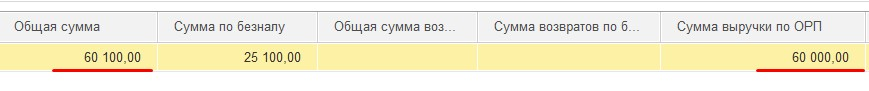
\includegraphics[width=1.0\textwidth]{12.jpg}
		\caption{<<Потерянный чек>>.}
		\label{ris:12.jpg}
	\end{figure}
	Здесь видно, что общая сумма  на 100 р. больше суммы выручки по ОРП.  (Рис.~\ref{ris:12.jpg})
	\item Первое, что  необходимо сделать - проверить по бумажным отчетом, что суммы внесены правильно. И если это действительно так и есть расхождения чисел, а не допущена ошибка ввода, приступаем к поискам потерянного чека.
	Нужно путем опроса кассиров или поиском в ОФД способом выяснить, какой товар был в этом чеке. . (Работа с сайтом ОФД изложена в п. \ref{5500})
	
	
	Установив товар в чеке или приняв решение чем его заменить нам нужно добавить этот чек в ОРП. Как  это сделать:
	
	\begin{itemize}
		\item Создать чек по нужной кассе. Записать его и с помощью ИТ отдела пересобрать ОРП.
		      Таким образом сумма выручки по ОРП сравняется с суммой по Z-отчету
	\end{itemize}
	
	
	
\end{itemize}
% Финансы

\newpage
\subsection{Формирование документа Возврат товаров поставщику}






\renewcommand{\arraystretch}{1.8} %% расстояние между строками таблицы
%\begin{landscape}
\begin{longtable}{|p{0.02\linewidth}|p{0.3\linewidth}|p{0.3\linewidth}|p{0.3\linewidth}|}
    %  {|c|c|l|c|}
    \hline
    № & \textbf{Действие} & \textbf{Ожидаемый результат} & \textbf{Фактический результат} \\
    %****************************************************************************************************
    \hline
    \hline
    \endhead
    \multicolumn{4}{|c|}{\textbf{\textit{Проверка на номенклатуру помеченную на удаление}}} \\
    \hline
    \hline
    \Rownum & Проверить, что включена константа <<крюПроверятьПомеченнуюНаУдалениеВДокументах>>  & &  \\
    \hline
    \Rownum &Перейти в раздел Закупки, выбрать <<Возвраты товаров поставщикам>>.  & 1. Открылся список документов  <<Возвраты товаров поставщикам>>;\par
    2. Отображаются все документы &  \\
    \hline
    \Rownum & Создать новый документ по кнопке \keys{Создать}  & 1. Открылась форма создания документа;\par
    2. По умолчанию в открывшейся форме заполнено поле <<Магазин>> &  \\
    \hline
    \Rownum & Заполнить реквизит <<Поставщик>> значением <<Метро>> &Заполнен <<Поставщик>> значением <<Метро>> ;    &  \\
    \hline
    \Rownum	& Нажать кнопку выбора складов & В форме выбора складов будет доступен только склад привязанный к текущему магазину  &  \\
    \hline
    \Rownum	& Выбрать склад & Заполнены реквизиты <<Склад>> и <<Организация>>  &  \\
    \hline
    \hline
    \Rownum	& Заполнить реквизит <<Причина возврата>> указав в качестве значения элемент выпадающего списка <<Возврат товара>> & Реквизит <<Причина возврата>> заполнен значением <<Возврат товара>> &  \\
    \hline
    \Rownum	& Нажать кнопку <<Добавить>> в табличной части <<Товары>>  & Откроется форма выбора справочника <<Номенклатура>>  &  \\
    \hline
    \Rownum	& Выбрать из справочника <<Номенклатура>> элемент помеченный на удаление & Заполнились поля в табличной части <<Код>>, <<Артикул>>, <<Номенклатура>>, <<Ед.изм>>, <<НДС>> &  \\
    \hline
    \Rownum	&Заполнить поле <<Количество>> значением <<1>>  & Заполнилось поле <<Количество>> &  \\
    \hline
    \Rownum	& Заполнить поле <<Цена>> значением <<1>>  & Заполнилось поле <<Цена>> &  \\
    \hline
    \Rownum	& Нажать кнопку \keys{Провести и закрыть} & 1. Программа выдает сообщение о неудачи проведения документа;\par 2. При закрытии окна сообщения в строке сообщений появляется текст ошибке с информацией, что документ содержит удаленную номенклатуру с указанием номеров строк и наименований &  \\
%****************************************************************************************************

%****************************************************************************************************

    %****************************************************************************************************

    %****************************************************************************************************
    \hline
    \hline
    \multicolumn{4}{|c|}{\textbf{\textit{Учет тары}}} \\
    \hline

    \hline
    \Rownum & Проверить, что включена константа <<крюПроводитьТару>>  & &  \\
    \hline
    \hline
    \Rownum &Перейти в раздел Закупки, выбрать <<Возвраты товаров поставщикам>>.  & 1. Открылся список документов  <<Возвраты товаров поставщикам>>;\par
    2. Отображаются все документы &  \\
    \hline
    \Rownum & Создать новый документ по кнопке \keys{Создать}  & 1. Открылась форма создания документа;\par
    2. По умолчанию в открывшейся форме заполнено поле <<Магазин>> &  \\
    \hline
    \Rownum & Заполнить реквизит <<Поставщик>> значением <<Метро>> &Заполнен <<Поставщик>> значением <<Метро>> ;    &  \\
    \hline
    \Rownum	& Нажать кнопку выбора складов & В форме выбора складов будет доступен только склад привязанный к текущему магазину  &  \\
    \hline
    \Rownum	& Выбрать склад & Заполнены реквизиты <<Склад>> и <<Организация>>  &  \\
    \hline
    \Rownum	& Заполнить реквизит <<Причина возврата>> указав в качестве значения элемент выпадающего списка <<Возврат кег>> & Реквизит <<Причина возврата>> заполнен значением <<Возврат кег>>  &  \\
    \hline
    \Rownum	& Нажать кнопку <<Добавить>> в табличной части <<Товары>>  & Откроется форма выбора справочника <<Номенклатура>>  &  \\
    \hline
    \Rownum	& Выбрать из справочника <<Номенклатура>> элемент с кодом <<00000013>> - <<КЕГ (50 л)>> & Заполнились поля в табличной части <<Код>>, <<Артикул>>, <<Номенклатура>>, <<Ед.изм>>, <<НДС>> &  \\
    \hline
    \Rownum	&Заполнить поле <<Количество>> значением <<1>>  & Заполнилось поле <<Количество>> &  \\
    \hline
    \Rownum	& Заполнить поле <<Цена>> значением <<1>>  & Заполнилось поле <<Цена>> &  \\
    \hline
    \Rownum	& Нажать кнопку \keys{Провести} &  Документ проводится без ошибок &  \\

    \hline
    \Rownum	& Выбрать команду <<Движения документа>> & Откроется отчет по движениям документа &  \\

    \hline
    \Rownum	& Найти в отчете движения по регистру <<Тара на складах>> & Движения документа по регистру накопления <<Тара на складах>> присутствуют. Измерения <<Период>>, <<Склад>>, <<Номенклатура>>, <<Поставщик>> заполнены. Значение ресурса <<Количество>> равно единице  &  \\
    \hline
    %****************************************************************************************************

    %****************************************************************************************************
    \hline
    \hline
    \multicolumn{4}{|c|}{\textbf{\textit{Очистка реквизита <<УчитыватьНДС>> и <<ЦенаВключаетНДС>>}}} \\

    \hline
    \Rownum & Проверить, что включена константа <<крюОчищатьНДСВВозвратеПоставщику>>  & &  \\

    \hline
    \Rownum &Перейти в раздел Закупки, выбрать <<Возвраты товаров поставщикам>>.  & 1. Открылся список документов  <<Возвраты товаров поставщикам>>;\par
    2. Отображаются все документы &  \\
    \hline
   \Rownum & Создать новый документ по кнопке \keys{Создать}  & 1. Открылась форма нового документа;\par
   2. По умолчанию в открывшейся форме заполнено поле <<Магазин>>\par
   3. Значение реквизитов <<ЦенаВключаетНДС>> и <<УчитыватьНДС>> на вкладке  <<Дополнительно>> равно <<Ложь>> &  \\
   \hline

    %****************************************************************************************************

     %****************************************************************************************************
    \hline
    \hline
    \multicolumn{4}{|c|}{\textbf{\textit{Печатная форма ТОРГ 12}}} \\
    \hline

    \hline
    \Rownum &Перейти в раздел Закупки, выбрать <<Возвраты товаров поставщикам>>.  & 1. Открылся список документов  <<Возвраты товаров поставщикам>>;\par
    2. Отображаются все документы &  \\
    \hline
    \Rownum & Открыть любой существующий документ  & 1. Открылась форма существующего документа;\par
     &  \\
     \hline
    \Rownum	& По кнопке выбора печатных форм выбрать <<ТОРГ-12(Товарная накладная на возврат)>>  & Сформировалась печатная форма &  \\
    \hline
    \Rownum	& Проверить представление организации и поле <<Вид операции>> в шапке & 1. В представлении организации присутствует КПП организации\par
    2. Поле <<Вид операции>> заполнено значением <<Возврат>>  &  \\


    %****************************************************************************************************





    \hline
    \Rownum	& test &  &  \\ %\nopagebreak Для запрещения разбиения страниц применяется команда \nopagebreak сразу после двух слешей в конце строчки.
    \hline
\end{longtable}
\newpage
\section{Возможные проблемы}

\begin{itemize}	
	\item  \stСитуация, когда на кассах будет разное время, достаточно нескольких секунд. И тогда какая-то из открытых смен может не попасть в УНФ, если по времени кассы она открылась раньше уже зафиксированной даты, а по текущему времени позже.

\end{itemize}
% ЕГАИС
\newpage
\section{РМК}
%\marginnote{\Date{Ср.}{08}{Апр.}{2020}}[-20pt]
\subsection{Алгоритмы РМК}


\begin{itemize}
	\item Реализована разбивка основного чека на два если присутствует номенклатура с разными системами налогообложения  (номенклатура находится в соответствующих номенклатурных группах)
	\item При подборе товара чек бокс <<остаток>> недоступен для редактирования, что днлает невозможным просмотр остатков при подборе
	\item  Алгоритм отключающий начисление бонусных баллов при покупке по карте <<Халва>> (расш.)
	\Nameref{513}
	\item Алгоритм логирующий этапы пробития чека ККМ , а так же алгоритм фиксации времени прохождения этапов набора, проведения и пробития чека
	\item При возникновении ошибок прежде чем пробивать новый чек, необходимо закончить работу со старым
	\item Алгоритм автоматического подбора тары при покупке разливного пива
	\item Изменена основная форма РМК, уменьшен размер
	\item Изменен шаблон вывода сообщения при превышении остатка на складе, теперь показывается только склад по которому превышен остаток и не показывается на какое количество
	\item Также при проверке отрицательных остатков, анализируется реквизит номенклатуры "ОтпускатьВМинус" и если он установлен, то дальнейшая проверка на отрицательные остаток не производится
	\item Перед началом оплаты, при установленной константе <<крюКонтрольСвоевременногоЗакрытияКассовойСмены>> проверяется, что если до закрытия кассовой смены осталось 10 мин и меньше, то выполняется запрет продажи
 	\item При установленной константе <<крюБлокировкаПараллельнойОплатыЭквайринг>> оплата по безналу одновременно на двух кассах блокируется
 	\item Если чек был разбит согласно технологии на два, а оплата была по безналу, то процедура возврата блокируется
 	\item Обработка РМК должна открываться только, если пользователь входит в группу "Кассиры"
 	\item Перед открытием смены выполняется закрытие эквайринговой смены ?
 	\item В форме меню, если есть необработанные чеки блокируются все элементы кроме "Регистрации продаж" и выходит сообщение с предложением разобраться с ошибками чеков
 	\item Если количество к продаже превышает остаток на складе, то в сообщении об ошибке не показывается на сколько превышение, а только склад по которому превышен остаток
 	\item Анализ чека на наличие в нем сообщения об ошибке
	\item Перед началом продаж кассиру показывается информационное сообщение с необходимостью поставить <<галочку>>, что он это сообщение прочел и понял
    \item Перед выполнением оплаты при включенной константе <<крюПроверятьОбъемПиваИБутылокВЧеке>> производится проверка соответствия объема разливных напитков и тары. Если есть несоответствие, то продажа блокируется


\end{itemize}


% РМК
\newpage
\subsection{Формирование документа Товарно-транспортная накладная ЕГАИС (входящая)}

\renewcommand{\arraystretch}{1.8} %% расстояние между строками таблицы
%\begin{landscape}
\begin{longtable}{|p{0.02\linewidth}|p{0.3\linewidth}|p{0.3\linewidth}|p{0.3\linewidth}|}
    %  {|c|c|l|c|}
    \hline
    № & \textbf{Действие} & \textbf{Ожидаемый результат} & \textbf{Фактический результат} \\
    %****************************************************************************************************
    \hline
    \hline
    \endhead
    \multicolumn{4}{|c|}{\textbf{\textit{******}}} \\
    \hline
    \hline

    %****************************************************************************************************


\end{longtable}% Табак
\newpage
\subsection{Регистрация дисконтных карт}
\subsubsection{Описание изменений в процессе регистрации дисконтных карт	}
\begin{itemize}	
	\item Изменения внесенные в процесс регистрации новой дисконтной карты. Теперь запись нового элемента справочника (новой дисконтной карты) произойдет только если будет указан верный вид дисконтной карты. Тот, который указан в настройках программы.
		\sidenote[-2ex][]{Есть возможность в настройках изменить тип карты}.
	\begin{figure}[H]
		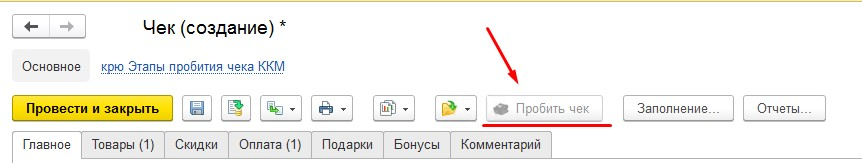
\includegraphics[width=0.8\textwidth]{30.jpg}
		\caption{Запрет записи.}
		\label{ris:30.jpg}
	\end{figure}

\end{itemize}% Сервис
\newpage
\subsection{Формирование документа Кассовая смена}

\renewcommand{\arraystretch}{1.8} %% расстояние между строками таблицы
%\begin{landscape}
\begin{longtable}{|p{0.02\linewidth}|p{0.3\linewidth}|p{0.3\linewidth}|p{0.3\linewidth}|}
    %  {|c|c|l|c|}
    \hline
    № & \textbf{Действие} & \textbf{Ожидаемый результат} & \textbf{Фактический результат} \\
    %****************************************************************************************************
    \hline
    \hline
    \endhead
    \multicolumn{4}{|c|}{\textbf{\textit{******}}} \\
    \hline
    \hline

    %****************************************************************************************************


\end{longtable}
\newpage
\section{Продажи}
\subsection{Объекты тестирования, описанные в разделе}

\begin{tabular}{p{0.05\linewidth}p{0.4\linewidth}p{0.4\linewidth}}
    \toprule
    %	\hline
    1 & Вид объекта & Документ \\
    \hline
    & Имя & ОтчетОРозничныхПродажах \\
    \hline
    & Синоним  & Отчет о розничных продажах \\
    \hline
    2 & Вид объекта  & Документ \\
    \hline
    & Имя & КассоваяСмена \\
    \hline
    & Синоним  & Кассовая смена \\
    \hline
    3 & Вид объекта  & Документ \\
    \hline
    & Имя & ВозвратТоваровОтПокупателя \\
    \hline
    & Синоним  & Возврат товаров от покупателя \\
    \hline

    \bottomrule %%% верхняя линейка
\end{tabular}
\newpage
\section{Справочники}
%\marginnote{\Date{Ср.}{08}{Апр.}{2020}}[-20pt]
\subsection{Номенклатура}

\begin{itemize}
	\item Изменение группы справочника "Номенклатура" блокируется в зависимости от установленной константы "крюИспользоватьБлокировкуНоменклатуры" и установки прав в РегистрСведений "крюПраваПользователей" (расш.)
	\Nameref{503}
	\item Изменение элемента справочника  "Номенклатура" блокируется в зависимости от установленной константы "крюИспользоватьБлокировкуНоменклатуры" и установки прав в РегистрСведений
	"крюПраваПользователей" блокируется не вся форма, а по определенному списку реквизитов и элементов управления
	(расш.) \Nameref{503}
	\item Блокировка реквизита "Артикул" вынесена отдельно и управляется константой "крюБлокироватьАртикул" 
	(расш.) \Nameref{503}	
\end{itemize}

\subsection{Организации}

\begin{itemize}

	\item Изменение элемента справочника  "Организации" блокируется при открытии в зависимости от установки прав в РегистрСведений "крюПраваПользователей" 
	(расш.) \Nameref{506}
	
\end{itemize}


\subsection{ФизическиеЛица}

\begin{itemize}
	
	\item Изменение элемента справочника  "Физические лица" блокируется при открытии в зависимости от установки прав в РегистрСведений "крюПраваПользователей" 
	(расш.) \Nameref{507}
	
\end{itemize}


\subsection{СтатьиДвиженияДенежныхСредств}

\begin{itemize}
	
	\item Изменение элемента справочника  "Статьи движения денежных средств" блокируется при записи в зависимости от установки значения константы "крюБлокироватьДДС" 
	(расш.) \Nameref{508}
	
\end{itemize}

 % Справочники
\newpage
% !TeX encoding = UTF-8
% !TeX spellcheck = russian_english
% !TeX root = Описание бизнес процессов.tex
\section{Дополнительные описания}

\subsection{Работа с весами}\label{1001}

Для решения задачи автоматической <<оттарки>> на весах, было сделано следующее:
Написана внешняя утилита-загрузчик по работе с весами <<Scales.exe>>. Утилита-загрузчик должна быть расположена в каталоге с базой данных.
Используется расширение \Nameref{512}.
В расширении после штатной загрузки весов происходит вызов  утилиты-загрузчика с помощью вызова штатной функции <<ЗапуститьПриложение>>, с передачей ей в командной строке:
\vspace{\baselineskip}

%\begin{itemize}
%	\item ПутьКФайлуЗагрузчика - Каталог с программой + имя файла утилиты-загрузчика
%	\item P\_RemoteHost - Адрес весов для обмена
%	\item P\_RemotePort - Порт весов для обмена
%	\item P\_TimeoutUDP - Таймаут 			 
%\end{itemize}
%\caption{Параметры коммандной строки}
\begin{tabular}{p{0.3\linewidth}p{0.3\linewidth}}
	\toprule   
	%	\hline
	Параметр & Значение \\
	\midrule
	ПутьКФайлуЗагрузчика & Каталог с программой + имя файла утилиты-загрузчика \\
%	\hline
	 P\_RemoteHost & Адрес весов для обмена \\
%	\hline
	 P\_RemotePort  & Порт весов для обмена \\
%	\hline
	 P\_TimeoutUDP  & Таймаут \\
%	\hline
	%	\hline
	\bottomrule %%% верхняя линейка
\end{tabular}


\vspace{\baselineskip}

Утилита-загрузчик читает данные из весов и на каждую запись (на каждое PLU) в весах создает пять дополнительных записей, в которых указан вес тары, а номер PLU увеличивается на 1000 с каждой тарой после первой, первая увеличивается на 2000, что бы оставить свободной первую тысячу номеров PLU. 

%\begin{itemize}
%	\item контейнер маленький  0,006г PLU +2000
%	\item контейнер средний    0,008г PLU +3000
%	\item контейнер большой    0,012г PLU +4000	
%	\item коробка фри          0,020г PLU +5000
%	\item пакет бумажный       0,015г PLU +6000	 
%\end{itemize}


\vspace{\baselineskip}
\begin{tabular}{p{0.3\linewidth}p{0.3\linewidth}}
	\toprule   
	%	\hline
	контейнер маленький & 0,006г PLU +2000 \\
%	\midrule
	контейнер средний & 0,008г PLU +3000 \\
	%	\hline
	контейнер большой & 0,012г PLU +4000 \\
	%	\hline
	коробка фри  & 0,020г PLU +5000 \\
	%	\hline
	пакет бумажный  & 0,015г PLU +6000 \\
	%	\hline
	%	\hline
	\bottomrule %%% верхняя линейка
\end{tabular}
\vspace{\baselineskip}


%\footnote{}
 Затем весы полностью очищаются и затем загружаются измененные данные.Если при загрузке весы не пустые, то загрузка останавливается.
 В случае если что то пошло не так (неполные данные в весах, отсутствие позиций и пр.) Нужно повторить выгрузку.
 
 
\subsection{Себестоимость номенклатуры}\label{1002}	 

В программе отключен штатный механизм расчета себестоимости. Расчет себестоимости производит ся в собственном общем модуле <<крюРасчетСебестоимости>>

В данные момент расчет себестоимости происходит при проведении следующих документов:  
\begin{itemize}
	\item Оприходование товаров
	\item Перемещение товаров
	\item Поступление товаров
	\item Сборка товаров
	
\end{itemize}

\subsection{Движение возвратной тары и оборудования}\label{1003}	 

Для решения задачи учета возвратной тары и оборудования создан новый регистр накопления <<ТараНаСкладах>>. 

Регистрация движений в регистре происходит при проведении следующих документов:  
\begin{itemize}
	\item Возврат товаров поставщику
	\item Поступление товаров
\end{itemize}

Для корректного отображения движения тары и оборудования, т.к. тара и оборудование могут придти только от конкретного поставщика и списание со склада может быть тоже только с указанием конкретного контрагента, то происходит блокировка проведения при наличии возвратной тары или оборудования в табличной части товары в  документах:

\begin{itemize}
	\item Перемещение товаров
	\item Оприходование товаров
	\item Приходный ордер на товары
	\item Расходный ордер на товары
\end{itemize}

Этот механизм реализован в общем модуле <<крюРасчетСебестоимости>>
	 

\subsection{Механизм сборки товаров}\label{1004}	 

Документ <<СборкаТоваров>> создается в момент проведения документа <<ОтчетОРозничныхПродажах>>.
Если документ <<ОтчетОРозничныхПродажах>> проводится повторно, то предварительно, ранее созданные документы <<СборкаТоваров>> на основании текущего, удаляются и создаются новые. Этот механизм позволяет актуализировать возможные изменения в документе <<ОтчетОРозничныхПродажах>>.

Документ <<СборкаТоваров>> создается на каждую строку номенклатуры табличной части <<Товары>>, документа  <<ОтчетОРозничныхПродажах>>, которая имеет запись в регистре сведений "КомплектующиеНоменклатуры" (кулинария).
Документ <<СборкаТоваров>> приходует на склад нужное количество комплектующих для корректной продажи конечной позиции номенклатуры. Так же в момент проведения документа <<СборкаТоваров>> расчитывается себестоимость итоговой позиции на основании себестоимости комплектующих.
При этом документ <<СборкаТоваров>> записывается по времени раньше, чем документ <<ОтчетОРозничныхПродажах>>. Это сделано для корректного списания остатков

\subsection{Помеченная на удаление номенклатура в документах}\label{1005}	 

Осуществляется проверка на наличие в табличной части <<Товары>> номенклатуры с пометкой удаления.
Выполняется в модуле <<крюРасчетСебестоимости>> для документов: 


\begin{itemize}
	\item Оприходование товаров
	\item Перемещение товаров
	\item Поступление товаров
	\item Списание товаров
	\item Приходный ордер на товары
	\item Расходный ордер на товары
	\item Возврат товаров поставщику
	
\end{itemize}

\subsection{Цены в документе Поступление товаров}\label{1006}	 

Перед проведением документа <<Поступление товаров>>, при установленной константе <<крюБлокировкаПродаж>>, выполняется проверка цен номенклатуры в табличной части <<Товары>>. Проверка на данном этапе не выполняется для следующих групп номенклатуры:
%\begin{itemize}
%	\item ЦБ-00005065 Сигареты без маркировки
%	\item ЦБ-00004758 Сигареты маркированные
%	\item КН000792 Кулинария
%\end{itemize}

\vspace{\baselineskip}
\begin{tabular}{p{0.3\linewidth}p{0.3\linewidth}}

	\toprule   
	ЦБ-00005065 & Сигареты без маркировки \\
	%	\midrule
	ЦБ-00004758 & Сигареты маркированные \\

	КН000792 & Кулинария \\
	\bottomrule %%% верхняя линейка
\end{tabular}
\vspace{\baselineskip}\par
Для проверки берется цена номенклатуры из регистра сведений <<крюЦеныНоменклатурыКонтрагентов>>,
которые устанавливаются специальным работником в разрезе магазина и контрагента и в случае использования характеристик номенклатуры - характеристики.\par
Если цена в документе оказывается больше чем установленная на данную номенклатуру в регистре или если цена на эту номенклатуру отсутствует, то в этом случае документ не проводится и формируется признак информационного сообщения. Если цена в документе ниже установленной в регистре, то формируется признак информационного сообщения.\par
После окончания проверки цен в табличной части документа, признак информационного  сообщения установлен, то информация по расхождению цен в документе отправляется по настроенным адресам электронной почты.\par
Адреса для отправки берутся из справочника <<УчетныеЗаписиЭлектроннойПочты>>, отбираются записи, у которых реквизит  <<ИмяПользователя>> содержит - <<КонтрольПТИУ>>.


\subsection{Документ перемещение, заполнение по виду цен}\label{1007}	 

В процедуре <<ПриСозданииНаСервере>>, при установленной константе <<крюСебестоимостьВПеремещении>>, отключается видимость элементов <<ТоварыЗаполнитьЦеныПоВидуЦен>> и <<ТоварыЗаполнитьЦеныПоРозничнымЦенам>>.
Далее создается команда и кнопка <<ЗаполнитьПоСебестоимости>>, при нажатии на которую цены в табличной части <<Товары>> заполняются по себестоимости.


\subsection{Документ ТТН Исходящая, на основании возврата}\label{1008}	 

Если документ <<Товарно-транспортная накладная ЕГАИС (исходящая)>> создается на основании<<Возврата товаров поставщику>>, то в расширении (расш.)
\Nameref{501} после процедуры <<ОбработкаЗаполнения>> вызывается штатная процедура <<ПрефиксацияОбъектовКлиентСервер.НомерНаПечать>>,которая из номера документа удаляет префикс и лидирующие нули.

\subsection{Контроль остатков алкогольной продукции}\label{1009}	 
%\renewcommand{\thefootnote}{\fnsymbol{footnote}}
В конфигурации создан регистр <<крюОстаткиАлкогольнойПродукцииТоргЗалЕГАИС>> для целей партионного учета алкогольной продукции. Регистр позволяет хранить остатки алкогольной продукции в торговом зале в разрезе справок В. \footnote{Тогда как при перемещении товара в регистр 2(Торговый зал) ЕГАИС справки В теряются} Это позволяет осуществлять корректные возвраты из регистра 2 с указанием конкретной Справки В по которой алкогольная продукция была передана в торговый зал. Упрощает создание возвратов поставщику, так можно выбрать по какой справке будем возвращать данную алкогольную продукцию. Позволяет легче решать проблемы с пересортицей товаров или возникшей ошибке продажи товара в минус. \par
\vspace{\baselineskip}\par
\vspace{\baselineskip}\par
Регистраторами у регистра являются следующие документы:
\begin{itemize}
	\item Акт постановки на баланс ЕГАИС
	\item Акт списания ЕГАИС
	\item Возврат из регистра №2 ЕГАИС
	\item Корректировка регистров
	\item Передача в регистр №2 ЕГАИС
\end{itemize}

\subsection{Акт списания, перезаполнение на основании ОРП}\label{1010}	 
%\renewcommand{\thefootnote}{\fnsymbol{footnote}}
На форму документа <<АктСписанияЕГАИС>>  добавлена кнопка \keys{Перезаполнить на основании ОРП} \par
Добавлена команда <<ЗаполнитьНаОснованииОРП>>, которая вызывает типовую процедуру <<ИнтеграцияЕГАИСРТ.ЗаполнитьАктСписанияЕГАИСНаОснованииОтчетаОРозничныхПродажах>>


\subsection{Документ <<Зарплата к выплате организаций>>}\label{1011}	 
В табличную часть <<Зарплата>> документа <<Зарплата к выплате организаций>> добавлен реквизит <<КлючСтроки>>. Данный реквизит заполняется обработкой по выдаче зарплаты, которая генерирует уникальный ключ строки и заполняет им реквизит. Это необходимо для механизма обмена с УТ10. В УТ на каждую строку документа создается РКО. <<КлючСтроки>> фиксируется в этом РКО, и по немк в случае перезагрузки документов из Розницы, происходит поиск и удаление документов РКО в УТ10.

\subsection{Цены в документе <<Установка цен номенклатуры>>}\label{1012}	 
% Дополнительные описания

\newpage
% !TeX root = Описание бизнес процессов.tex
% !TeX encoding = UTF-8
% !TeX spellcheck = russian_english
\appendix
\titleformat{\section}[display]
{\normalfont\Large\bfseries}
{\centering Приложение\ \thesection\\(справочное)}
{0pt}{\Large\centering}
\renewcommand{\thesection}{\Asbuk{section}}

\section{Приложение: Константы и их описание}
 Список констант добавленных в конфигурацию с типом и  описанием  их назначения:\par
\begin{enumerate}[label=(\arabic*)]

\vspace{\baselineskip}
\item \textbf{\textit{крюДатаЗапретаПроведенияДокументовБезТранспортнойТары}}
\begin{description}
	\item[Тип] : Дата
	\item[Использование] : Дата начала запрета проведения документов без транспортной тары
\end{description}
\vspace{\baselineskip}
\item \textbf{\textit{крюДополнительныеЗначенияМагазинКПП}}
\begin{description}
	\item[Тип] : ПланВидовХарактеристик
	\item[Использование] : Использование в конфигурации и расширениях не обнаружено
\end{description}
\vspace{\baselineskip}
\item \textbf{\textit{крюГраницаПоследовательностиУстановкиСебестоимости}}
\begin{description}
	\item[Тип] : Дата
	\item[Использование]: Использование в конфигурации и расширениях не обнаружено
\end{description}

\vspace{\baselineskip}
\item \textbf{\textit{крюИспользоватьАвтонумерациюАртикула}}
\begin{description}
	\item[Тип] : Число
	\item[Использование]: Включает использование собственного нумератора
\end{description}

\vspace{\baselineskip}
\item \textbf{\textit{крюБлокироватьАртикул}}
\begin{description}
	\item[Тип] : Булево
	\item[Использование]: Отвечает за блокировку артикула
\end{description}

\vspace{\baselineskip}
\item \textbf{\textit{крюИспользоватьБлокировкуНоменклатуры}}
\begin{description}
	\item[Тип] : Булево
	\item[Использование]: Отвечает за блокировку справочника <<Номенклатура>>
\end{description}

\vspace{\baselineskip}
\item \textbf{\textit{крюИспользоватьБлокировкуВводаНовогоНоментклатуры}}
\begin{description}
	\item[Тип] : Булево
	\item[Использование]: Использование в конфигурации и расширениях не обнаружено
\end{description}


\vspace{\baselineskip}
\item \textbf{\textit{крюПроверятьЦеныПоставщика}}
\begin{description}
	\item[Тип] : Булево
	\item[Использование]: Использование в конфигурации и расширениях не обнаружено
\end{description}

\vspace{\baselineskip}
\item \textbf{\textit{крюПогрешность}}
\begin{description}
	\item[Тип] : Число
	\item[Использование]: Использование в конфигурации и расширениях не обнаружено
\end{description}

\vspace{\baselineskip}
\item \textbf{\textit{крюКонтролироватьДисконтКарты}}
\begin{description}
	\item[Тип] : Булево
	\item[Использование]: Устанавливает контроль за созданием дисконтных карт
\end{description}

\vspace{\baselineskip}
\item \textbf{\textit{крюДисконтКартаДляВыбора}}
\begin{description}
	\item[Тип] : СправочникСсылка.ВидыДисконтныхКарт
	\item[Использование]: Устанавливает разрешенный для создания вид дисконтных карт
\end{description}

\vspace{\baselineskip}
\item \textbf{\textit{крюКонролироватьПроведениеОРП}}
\begin{description}
	\item[Тип] : Булево
	\item[Использование]: Контролировать или нет при проведении ОРП в узле проводят документ или в ЦУ
\end{description}


\vspace{\baselineskip}
\item \textbf{\textit{крюИнфоТекстДляМагазина}}
\begin{description}
	\item[Тип] : Строка
	\item[Использование]: Информация для печати в чеке
\end{description}

\vspace{\baselineskip}
\item \textbf{\textit{крюИнфоТекстДляКассира}}
\begin{description}
	\item[Тип] : Строка
	\item[Использование]: Содержит информацию, которая показывается кассиру перед запуском рабочего места (перед началом продаж)
\end{description}


\vspace{\baselineskip}
\item \textbf{\textit{крюВыполнятьПроверкуМинимальныхОстатков}}
\begin{description}
	\item[Тип] : Булево
	\item[Использование]: Запускать или нет обработку по проверке минимальных остатков ключевых позиций при старте системы
\end{description}


\vspace{\baselineskip}
\item \textbf{\textit{крюКонтролироватьВозвратнуюТару}}
\begin{description}
	\item[Тип] : Булево
	\item[Использование]: Определяет выполнять ли контроль на наличие возвратной тары в документе
\end{description}


\vspace{\baselineskip}
\item \textbf{\textit{крюПроводитьТару}}
\begin{description}
	\item[Тип] : Булево
	\item[Использование]: Отвечает за движения по регистру <<ТараНаСкладах>>
\end{description}

\vspace{\baselineskip}
\item \textbf{\textit{крюДатаНачалаУчетаКег}}
\begin{description}
    \item[Тип] : Дата
    \item[Использование]: Дата с которой начинаем учитывать движение тары
\end{description}

\vspace{\baselineskip}
\item \textbf{\textit{крюПроверятьОбработкуЧековККМ}}
\begin{description}
    \item[Тип] : Булево
    \item[Использование]: Проверять ли наличие не проведенных чеков
\end{description}

\vspace{\baselineskip}
\item \textbf{\textit{крюПроверятьОбъемПиваИБутылокВЧеке}}
\begin{description}
    \item[Тип] : Булево
    \item[Использование]: Проверять ли в чеке соответствие объема разливных напитков и объема тары
\end{description}

\vspace{\baselineskip}
\item \textbf{\textit{крюОтправлятьАктыЕГАИСПриЗакрытииСмены}}
\begin{description}
    \item[Тип] : Булево
    \item[Использование]: Выполнять отправку Актов списания ЕГАИС срразу при закрытии смены или нет
\end{description}

\vspace{\baselineskip}
\item \textbf{\textit{крюДопПроверкаОстатковНоменклатурыПриПроведенииОРП}}
\begin{description}
    \item[Тип] : Булево
    \item[Использование]: Если константа установлена в <<Ложь>>, то при проверке отрицательных остатков при проведении ОРП, берется только номенклатура с реквизитом <<ОтпускатьВМинус>> = <<Ложь>>. Т.е. контроль только номенклатуры, которую запрещено продавать в минус.
\end{description}

\vspace{\baselineskip}
\item \textbf{\textit{крюПомещатьНепробитыйЧекВПеременную}}
\begin{description}
    \item[Тип] : Булево
    \item[Использование]: Разрешает фиксировать ссылку на не пробитый чек в реквизите формы РМК
\end{description}


\vspace{\baselineskip}
\item \textbf{\textit{крюСинхронизацияТолькоМонопольно}}
\begin{description}
    \item[Тип] : Булево
    \item[Использование]: Устанавливает режим монопольной синхронизации
\end{description}

\vspace{\baselineskip}
\item \textbf{\textit{крюЧасЗапретаСинхронизации}}
\begin{description}
    \item[Тип] : Число
    \item[Использование]: Устанавливает время с котрого запрещена синхронизация
\end{description}


\vspace{\baselineskip}
\item \textbf{\textit{крюДокументыЗакрытияСменыРавныДатеНачалаСмены}}
\begin{description}
    \item[Тип] : Булево
    \item[Использование]: Будут ли у документов закрытия смены устанавливаться дата началом смены
\end{description}



\vspace{\baselineskip}
\item \textbf{\textit{крюТекстБлокировкаПродаж}}
\begin{description}
    \item[Тип] : Строка
    \item[Использование]: Механизм не работал. Был переписан. Включается константой <<крюЗакрытияКассовойСмены\_Монопольно>>
\end{description}


\vspace{\baselineskip}
\item \textbf{\textit{крюБлокировкаПродаж}}
\begin{description}
    \item[Тип] : Булево
    \item[Использование]: Механизм не работал. Был переписан. Включается константой <<крюЗакрытияКассовойСмены\_Монопольно>>
\end{description}

\vspace{\baselineskip}
\item \textbf{\textit{крюПопыткиПроводитьПробитыйЧек}}
\begin{description}
    \item[Тип] : Булево
    \item[Использование]: Делать или нет попытки многократного проведения чека (для чего?)
\end{description}


\vspace{\baselineskip}
\item \textbf{\textit{крюОтчетБезГашенияПоЭквайрингу}}
\begin{description}
    \item[Тип] : Булево
    \item[Использование]: Разрешить выводить отчет без гашения по эквайрингу
\end{description}



\vspace{\baselineskip}
\item \textbf{\textit{крюРазделениеПоСобственнойТаре}}
\begin{description}
    \item[Тип] : Булево
    \item[Использование]: Указывать или нет в чеке собственную тару, если да то в чек добавляется строчка <<Налито в собственную потребительскую тару>>
\end{description}

\vspace{\baselineskip}
\item \textbf{\textit{крюУбратьАвтоСкидкиВПервомЧеке}}
\begin{description}
    \item[Тип] : Булево
    \item[Использование]: Очищать или нет поля <<СуммаАвтоматическойСкидки>> и <<ПроцентАвтоматическойСкидки>> в чеке
\end{description}


\vspace{\baselineskip}
\item \textbf{\textit{крюБлокировкаПродажПослеДвенадцати}}
\begin{description}
    \item[Тип] : Булево
    \item[Использование]: Регулирует запрет продаж после 00-00
\end{description}

\vspace{\baselineskip}
\item \textbf{\textit{крюКонтролироватьСубконто}}
\begin{description}
    \item[Тип] : Булево
    \item[Использование]: Если контролировать, то проверяется наличие статьи ДДС в табличной части <<РасшифровкаПлатежа>> документа <<РасходныйКассовыйОрдер>> и соответствие этой статьи определенному списку
\end{description}

\vspace{\baselineskip}
\item \textbf{\textit{крюБлокироватьДДС}}
\begin{description}
    \item[Тип] : Булево
    \item[Использование]: Если блокировка включена, то при попытке записи элемента справочника <<СтатьиДвиженияДенежныхСредств>> происходит отказ от записи
\end{description}


\vspace{\baselineskip}
\item \textbf{\textit{крюЗапретВозвратаНаДругойКассе}}
\begin{description}
    \item[Тип] : Булево
    \item[Использование]: Запрещает возврат по другой кассе
\end{description}


\vspace{\baselineskip}
\item \textbf{\textit{крюВозвратВПределахСмены}}
\begin{description}
    \item[Тип] : Булево
    \item[Использование]: Разрешает проводить возврат, только в пределах смены в которой был пробит чек
\end{description}


\vspace{\baselineskip}
\item \textbf{\textit{крюОчищатьНДСВВозвратеПоставщику}}
\begin{description}
    \item[Тип] : Булево
    \item[Использование]: При установленной константе очищает устанавливает в <<Ложь>> реквизиты <<УчитыватьНДС>> и <<ЦенаВключаетНДС>> в документе <<ВозвратТоваровПоставщику>>
    \begin{myquote}
        Проверить как это соотносится с механизмом НДС с КХН
    \end{myquote}
\end{description}



\vspace{\baselineskip}
\item \textbf{\textit{крюРазделительТиреВПКО}}
\begin{description}
    \item[Тип] : Булево
    \item[Использование]: При установленной константе в макете инкассации в РКО в сумме цифрами, запятая заменяется на тире
\end{description}


\vspace{\baselineskip}
\item \textbf{\textit{крюПечатьРКОСразуНаПринтер}}
\begin{description}
    \item[Тип] : Булево
    \item[Использование]: При установленной константе печатный формы инкассации в РКО отправляются на принтер без предварительного просмотра
\end{description}

\vspace{\baselineskip}
\item \textbf{\textit{крюПодотчетПКОНаОсновании}}
\begin{description}
    \item[Тип] : Булево
    \item[Использование]: Для создания ПКО для возврата подотчета
\end{description}


\vspace{\baselineskip}
\item \textbf{\textit{крюКонтролироватьПКОПодотчет}}
\begin{description}
    \item[Тип] : Булево
    \item[Использование]: Если ПКО подотчет (возврат из подотчета), то без документа основания не проводить
\end{description}


\vspace{\baselineskip}
\item \textbf{\textit{крюПроверятьГТД}}
\begin{description}
    \item[Тип] : Булево
    \item[Использование]: Включает проверку ГТД (Не используется в текущий момент)
\end{description}

\vspace{\baselineskip}
\item \textbf{\textit{крюДатаНачалаПроверкиГТД}}
\begin{description}
    \item[Тип] : Дата
    \item[Использование]: Дата начала проверки ГТД (Не используется в текущий момент)
\end{description}

\vspace{\baselineskip}
\item \textbf{\textit{крюКоличествоСимволовГТД}}
\begin{description}
    \item[Тип] : Дата
    \item[Использование]: Количество символо при проверке ГТД (Не используется в текущий момент)
\end{description}

\vspace{\baselineskip}
\item \textbf{\textit{крюВерсияПротоколоЕГАИС}}
\begin{description}
    \item[Тип] : Дата
    \item[Использование]: Содержит версию протокола ЕГАИС для обмена с УТМ (Не используется в текущий момент)
\end{description}

\vspace{\baselineskip}
\item \textbf{\textit{крюВерсияПротоколоЕГАИС}}
\begin{description}
    \item[Тип] : Число
    \item[Использование]: Содержит версию протокола ЕГАИС для обмена с УТМ (Не используется в текущий момент?)
\end{description}

\vspace{\baselineskip}
\item \textbf{\textit{крюШаблонНетГТД}}
\begin{description}
    \item[Тип] : Строка
    \item[Использование]: Содержит строку шаблона для проверки ГТД (Не используется в текущий момент)
\end{description}

\vspace{\baselineskip}
\item \textbf{\textit{крюРазделениеПоКулинарии}}
\begin{description}
    \item[Тип] : Булево
    \item[Использование]: Управляет разделением на два чека кулинария и все остальное
\end{description}

\vspace{\baselineskip}
\item \textbf{\textit{КрюРазрешитьНесколькоККМ}}
\begin{description}
    \item[Тип] : Булево
    \item[Использование]: Разрешает использование виртуальных касс
\end{description}

\vspace{\baselineskip}
\item \textbf{\textit{крюТекущийМагазин}}
\begin{description}
    \item[Тип] : СправочникСсылка.Магазины
    \item[Использование]: Сохраняет текущий магазин для различных обработок
\end{description}

\vspace{\baselineskip}
\item \textbf{\textit{КрюОпросКассираПриОкончанииСмены}}
\begin{description}
    \item[Тип] : Булево
    \item[Использование]: Выполнять или нет опрос кассиров при закрытии смены (внесение чисел с чека для контроля)
\end{description}

\vspace{\baselineskip}
\item \textbf{\textit{КрюОпросКассировСравниватьБезнал}}
\begin{description}
    \item[Тип] : Булево
    \item[Использование]: Выполнять или нет сравнение данных по безналу при закрытии смены
\end{description}

\vspace{\baselineskip}
\item \textbf{\textit{КрюОпросКассировСравниватьОРП}}
\begin{description}
    \item[Тип] : Булево
    \item[Использование]: Выполнять или нет сравнение данных по налу при закрытии смены
\end{description}

\vspace{\baselineskip}
\item \textbf{\textit{КрюДопПроведениеОРП}}
\begin{description}
    \item[Тип] : Булево
    \item[Использование]: Выполнять или нет доп проведение ОРП (не очень ясно)
\end{description}

\vspace{\baselineskip}
\item \textbf{\textit{крюВключитьБлокировкуПараллельнойОплатыЭквайринг}}
\begin{description}
    \item[Тип] : Булево
    \item[Использование]: При установленной константе блокируется одновременная оплата по безналу на разных кассах
\end{description}

\vspace{\baselineskip}
\item \textbf{\textit{крюБлокировкаПараллельнойОплатыЭквайринг}}
\begin{description}
    \item[Тип] : Булево
    \item[Использование]: Связана с константой <<крюВключитьБлокировкуПараллельнойОплатыЭквайринг>>
\end{description}


\vspace{\baselineskip}
\item \textbf{\textit{крюКопироватьФайлТерминала}}
\begin{description}
    \item[Тип] : Булево
    \item[Использование]: При установленной константе <<p-файл>> с текстом текущего чека, копируется в служебный каталог
\end{description}

\vspace{\baselineskip}
\item \textbf{\textit{крюЗаменитьНедопустимыеСимволыСбербанк}}
\begin{description}
    \item[Тип] : Булево
    \item[Использование]: При установленной константе заменяет недопустимые символы в XML при печати чека
\end{description}

\vspace{\baselineskip}
\item \textbf{\textit{крюОплатаБезСложнойФорсы}}
\begin{description}
    \item[Тип] : Булево
    \item[Использование]: Константа включает доработку в обработке <<РМКУправляемыйРежим>>.
    Изменения касаются оплаты. Отключена сложная оплаты. Из основного интерфейса спрятаны кнопки нал, базнал оплат.
\end{description}

\vspace{\baselineskip}
\item \textbf{\textit{крюПроверкаФормированияЧековККМ\_РМКУправляемыйРежим}}
\begin{description}
    \item[Тип] : Булево
    \item[Использование]: Управляет процедурой проверки чеков (???)
\end{description}

\vspace{\baselineskip}
\item \textbf{\textit{крюИспользоватьНовыйМеханизмДеленияЧековККМ}}
\begin{description}
    \item[Тип] : Булево
    \item[Использование]:  По данной константе запускается переписанный механизм дробления чеков. Чтоб чеки в любом случае записывалась. Если все работает хорошо процедуру <<ПробитьЧекККМСложныйСлучайЗавершение>> можно будет удалить полностью.
\end{description}

\vspace{\baselineskip}
\item \textbf{\textit{крюСебестоимостьВПеремещении}}
\begin{description}
    \item[Тип] : Булево
    \item[Использование]: Управляет механизмом выбора вида цен для заполнения в <<ПеремещениеТоваров>>
\end{description}

\vspace{\baselineskip}
\item \textbf{\textit{крюСверкаИтоговСЗакрытиемЭквайрингаДоОпросаКассира}}
\begin{description}
    \item[Тип] : Булево
    \item[Использование]: Участвует в механизме опроса кассиров
\end{description}


\vspace{\baselineskip}
\item \textbf{\textit{крюЗакрытияКассовойСмены\_Монопольно}}
\begin{description}
    \item[Тип] : Булево
    \item[Использование]: Включает механизм, разделяющий продажу и закрытия смены.
    Если идет продажа закрытия смены ожидает и наоборот
\end{description}

\vspace{\baselineskip}
\item \textbf{\textit{крюКонтрольСвоевременногоЗакрытияКассовойСмены}}
\begin{description}
    \item[Тип] : Булево
    \item[Использование]: Включает механизм контроля оставшегося времени на открытой кассе (не должно превышать 24ч). За 30 мин. до истечения включается оповещения кассира. За 10 мин. до истечения блокируется возможность продажи
\end{description}

\vspace{\baselineskip}
\item \textbf{\textit{КрюЗапретВозвратаПоЭквайрингуРазбитыхЧеков\_Кулинария}}
\begin{description}
    \item[Тип] : Булево
    \item[Использование]: Блокировка возврата если чек был разбит по кулинарии, и вид оплаты безнал
\end{description}


\vspace{\baselineskip}
\item \textbf{\textit{крюПроверятьПомеченнуюНаУдалениеВДокументах}}
\begin{description}
    \item[Тип] : Булево
    \item[Использование]: Проверять или нет помеченную на удаление номенклатуру в документа в ТЧ Товары
\end{description}


\vspace{\baselineskip}
\item \textbf{\textit{КрюКоличествоОбрабатываемыхЗаписей\_РегламентнаяСверткаБонусныеБаллы}}
\begin{description}
    \item[Тип] : Булево
    \item[Использование]: Регламентное задание отключено при константе равной 0.
    Указывается количество обрабатываемых дисконтных карт за один цикл регламентного задания
\end{description}

\vspace{\baselineskip}
\item \textbf{\textit{КрюДисконтныйСервер\_ВключитьПроверкуСоединения}}
\begin{description}
    \item[Тип] : Булево
    \item[Использование]: Включает проверку доступности дисконтного сервера раз в 10 мин
\end{description}

\vspace{\baselineskip}
\item \textbf{\textit{КрюДисконтныйСервер\_Адрес}}
\begin{description}
    \item[Тип] : Строка
    \item[Использование]: Адрес дисконтного сервера который будет пинговаться
\end{description}

\vspace{\baselineskip}
\item \textbf{\textit{КрюДисконтныйСервер\_ИнтервалОпросаДисконта}}
\begin{description}
    \item[Тип] : Число
    \item[Использование]: Интервал опроса дисконтного сервера
\end{description}





\end{enumerate}

%\begin{dot2tex}[neato,mathmode]
%    digraph G {
%        node [shape="circle"];
%        a\_1 -> a\_2 -> a\_3 -> a\_4 -> a\_1;
%    }
%\end{dot2tex} % Описание прочих изменений
%\newpage
\newpage
\section{Приложение: Места с изменениями}
 Список процедур и функций с внесенными изменениями:\par

\paragraph{При открытии документа корректно заполняется значение глобальной переменной НомерДокументаКассыККМ}\label{2001}
\begin{itemize}
    \item Документ.ВозвратТоваровОтПокупателя.Форма.ФормаДокумента.Форма.Модуль
    \textbf{Процедура <<ПриОткрытии>>}
     \item Документ.ВозвратТоваровОтПокупателя.Форма.ФормаДокумента.Форма.Модуль
    \textbf{Процедура <<КассаККМПриИзмененииКлиент>>}
    \item Документ.ВозвратТоваровОтПокупателя.Форма.ФормаДокумента.Форма.Модуль
   \textbf{ Процедура <<НапечататьЧекКлиент>>}
     \item Документ.ВозвратТоваровОтПокупателя.Форма.ФормаДокумента.Форма.Модуль
    \textbf{Процедура <<НапечататьЧекКлиентЗавершение>>}
\end{itemize} % Описание прочих изменений
%\newpage
%\listoffigures
%\newpage

%\addcontentsline{toc}{chapter}{Index}

%\newpage

%\printglossary



\begin{versionhistory}
	\vhEntry{0.01}{11.05.20}{PK}{Добавлены схемы}
    \vhEntry{0.10}{11.05.20}{PK}{Добавлено описание и настройка}
    \vhEntry{0.20}{11.05.20}{PK}{Добавлено описание расширений}
    \vhEntry{0.25}{13.05.20}{PK}{Расширено описание}

\end{versionhistory}
%\vhListAllAuthorsLong % Список авторов
%\newpage
%\listoftodos
%\printindex
%\listoftodos[Необходимые правки]
%\printindex % печать предметного указателя здесь
\end{document}
